\documentclass[11pt]{article}
\usepackage{../ee16}
\usepackage{../markup}
\usepackage{changepage}
\usepackage{tikz}
\usetikzlibrary{calc}
\usepackage{color,hyperref,listings,enumitem}
\usepackage{algorithm}
\usepackage{algpseudocode}
\usepackage{tkz-euclide}
\usepackage{physics}
\usepackage{multicol}
\usepackage{pgfplots}
\usepackage{adjustbox}
\usepackage{cancel}
\usepackage{commath}
\usepackage{mathdots}
\usepackage[american,siunitx]{circuitikz}
\sisetup{per-mode=fraction}
\sisetup{quotient-mode=fraction}
\DeclareSIUnit \decade {dec}
\lstset{basicstyle=\ttfamily}
\newcommand{\fillin}[1]{\underline{\hskip #1}}
\newcommand{\doublehrule}{\hrule \vskip 0.02in \hrule}
\newcommand*\circled[1]{\tikz[baseline=(char.base)]{
  \node[shape=circle,draw,inner sep=2pt] (char) {#1};}}

\definecolor{blueish}{rgb}{0.7,0.1,.7}
\newcommand{\sol}[1]{{\color{blueish} \textbf{Solution: } #1}} % solutions in pink
\newcommand{\ws}[1]{} % worksheet exclusive material
\newcommand{\meta}[1]{{\vspace{2pt} \color{blue} \textbf{Meta: } #1}} % for meta in blue

\input{../../newcommands/newcommands-eg-ie-etc}
\input{../../newcommands/newcommands-labels-refs}
\input{../../newcommands/newcommands-math}


\begin{document}

\def\title{Worksheet 1}

\newcommand{\qitem}{\qpart\item}

\renewcommand{\labelenumi}{(\alph{enumi})} % change default enum format to (a)
\renewcommand{\theenumi}{(\alph{enumi})} % fix reference format accordingly.
\renewcommand{\labelenumii}{\roman{enumii}.} % second level labels.
\renewcommand{\theenumii}{\roman{enumii}.}

\maketitle

\vspace{0.5em}

\begin{qunlist}

% Authors: Son Tran, Naomi Sagan, Taejin Hwang
% Emails: sontran@berkeley.edu, naomi.sagan@berkeley.edu, taejin@berkeley.edu

\qns{Change of Coordinates}

Many engineering problems can be difficult to solve in its standard xyz coordinates, but may be much easier in a different coordinate system.
In this set, we will review the process of \textbf{change of basis} between coordinate systems.
Remember that a \emph{change of basis} can be represented by a invertible, square matrix. \vskip 1pt
Let's first start with an example:
Consider the vector $\vec{x} = \begin{bmatrix} x_1 \\ x_2 \end{bmatrix}.$ 
When we write a vector in this form, we are implicitly representing it with the \textbf{standard basis} for $\R^{2}$, $\vec{e_1} = \begin{bmatrix} 1 \\ 0 \end{bmatrix}$ and $\vec{e_2} = \begin{bmatrix} 0 \\ 1 \end{bmatrix}.$ \vspace{1em} 
This means that we can write $\vec{x}$ as a linear combination using standard basis vectors $\vec{x} = x_1\vec{e_1} + x_2\vec{e_2}$. \vspace {1em} 
Now, what if we want to represent $\vec{x}$ as a linear combination of another set of basis vectors, say $\vec{v_1} = \begin{bmatrix} 1 \\ 1 \end{bmatrix}$ and $\vec{v_2} = \begin{bmatrix} 0 \\ -1 \end{bmatrix}?$ \vskip 1pt
This means that we need to find scalars $\alpha_{1}$ and $\alpha_{2}$ such that $\vec{x} = \alpha_1 \vec{v_1} + \alpha_2 \vec{v_2}$.
We can write this equation in matrix form:
\[
  \begin{bmatrix}
    | & | \\
    \vec{v_1} & \vec{v_2} \\
    | & |
  \end{bmatrix}
  \begin{bmatrix} \alpha_1 \\ \alpha_2 \end{bmatrix} = \begin{bmatrix} x_1 \\ x_2 \end{bmatrix}
.\]

Or equivalently:
\[
  \begin{bmatrix}
    1 & 0 \\
    1 & -1
  \end{bmatrix}
  \begin{bmatrix} \alpha_1 \\ \alpha_2 \end{bmatrix} = \begin{bmatrix} x_1 \\ x_2 \end{bmatrix}
.\]
Thus we can find $\alpha_1$ and $\alpha_2$ by solving a system of linear equations as seen in 16A. \\
These scalars $\alpha_1$ and $\alpha_2$ are called the coordinates of $\vec{x}$ \textbf{in the basis} $S = \{\vec{v_1}, \vec{v_2} \}.$

For the following problems, we will look at a vector $\vec{x}$ currently in the standard basis 
and its representation in a different basis: $S = \{\vec{v_1}, \vec{v_2} \}.$ \vskip 4pt
We will refer to the vector $\vec{x}$ using coordinates from the basis $S$ as $[\vec{x}]_S.$ In other words, \vskip 3pt 
if $\vec{x} = \begin{bmatrix} x_1 \\ x_2 \end{bmatrix},$ and $[\vec{x}]_S = \begin{bmatrix} \alpha_1 \\ \alpha_2 \end{bmatrix},$ then $\vec{x} = x_1 \vec{e_1} + x_2 \vec{e_2}$ or $\vec{x} = \alpha_1 \vec{v_1} + \alpha_2 \vec{v_2}.$

\begin{enumerate}
  % Part(a)
  \qitem Now let's say we have a vector that is originally using coordinates from the basis S. 
  That is $[\vec{x}]_S = \begin{bmatrix} 3 \\ 3 \end{bmatrix}.$ We are told that the basis S is:
  \begin{gather*}
    \vec{v_1} =
    \begin{bmatrix}
      1 \\
      1
    \end{bmatrix},
    \vec{v_2} = \begin{bmatrix}
      1 \\
      -1
    \end{bmatrix}
  \end{gather*}
  What equation gives the coordinates of $\vec{x}$ in the standard basis?

  % Part(a) solution
  \sol{
    Since the vector $\vec{x}$ is currently written in coordinates using the basis, $S = \{\vec{v_1}, \vec{v_2} \},$
    we know that $\vec{x} = 3 \begin{bmatrix} 1 \\ 1 \end{bmatrix} + 3 \begin{bmatrix} 1 \\ -1 \end{bmatrix} = V [\vec{x}]_S$
    where $V$ is the matrix $\begin{bmatrix} 1 & 1 \\ 1 & -1 \end{bmatrix}.$ Therefore,
    $$
    \vec{x} =
    \begin{bmatrix}
      1 & 1 \\
      1 & -1
    \end{bmatrix}
    \begin{bmatrix}
      3 \\
      3
    \end{bmatrix}
    $$
  }

  % Part(b)
  \qitem Let $\vec{x} = \begin{bmatrix} 2 \\ -1 \end{bmatrix}$. What equation gives the coordinates of $\vec{x}$ in the basis S? 
  Try to express your answer in matrix-vector form. No need to do the full calculation.
  \begin{gather*}
    \vec{v_1} =
    \begin{bmatrix}
      4 \\
      -2
    \end{bmatrix},
    \vec{v_2} = \begin{bmatrix}
      -3 \\
      -3
    \end{bmatrix}
  \end{gather*}
  What equation gives the coordinates of $\vec{v}$ in the standard basis?

  % Part(b) solution
  \sol {
    If we denote the vector in the new basis as $[\vec{x}]_S = \begin{bmatrix} \alpha_1 \\ \alpha_2 \end{bmatrix}$, then we can write out the following equation: $\vec{x} = \alpha_1 \vec{v_1} + \alpha_2 \vec{v_2} = V [\vec{x}]_S$ where V is the same matrix used in the previous part. Then it follows that $[\vec{x}]_S = V^{-1} \vec{x}.$
  }

  \end{enumerate}

  Now that we've had some mechanical practice, we'll look at the representation of linear operators through different bases. 
  For a linear transformation, we can represent the input-output relationship with the matrix vector equation:
  $\vec{y} = A \vec{x}$ where $\vec{x}$ is the input, and $\vec{y}$ is the output vector.
  In this question we will look at how the linear operator represented by the matrix $A$ looks in a \textit{different basis} $S.$
  Remember that the vector $\vec{x}$ is implicitly written in the \textbf{standard basis} while the vector $[\vec{x}]_S$ is a vector using coordinates from the \textbf{S-basis.}

  \begin{enumerate}[resume]
  %part c
  \qitem Let $[\vec{x}]_S$ be a vector using $S$ coordinates, and $V$ be a change of coordinates matrix from the $S$-basis to the standard basis. \\
  How can we represent $[\vec{x}]_S$ in terms of $\vec{x}$ and $V?$
  \sol {
    We are given a matrix $V$ that converts $S$ coordinates to standard coordinates. 
    This means that $V^{-1}$ will be the matrix that converts standard coordinates to the $S$ coordinates.
    Therefore, in order to get $[\vec{x}]_S$ we multiply $V^{-1}$ with $\vec{x},$ to get
    $V^{-1} \vec{x} = [\vec{x}]_S.$
  }

  % Part(d)
  \qitem Now suppose we have another basis $R = \{w_1, .. , w_n\}$ and the change of basis from $R$ to $S$ is represented by the matrix $W.$ This means that if we have a vector $[\vec{x}]_R$ in R-coordinates, to get the coordinate representation in S-coordinates, $[\vec{x}]_S = W[\vec{x}]_R.$ What would the change of basis matrix that takes a vector in $R$ coordinates and outputs a vector in standard coordinates look like?
  \sol {
    We want to get represent the vector $\vec{x}$ in standard coordinates.
    We are looking for a matrix $U$ such that
    $$\vec{x} = U [\vec{x}]_R.$$
    We currently know that in order to go from S-coordinates to standard, we must multiply by the matrix $V.$
    $$\vec{x} = V [\vec{x}]_S.$$
    We also know that to go from R-coordinates to S-coordinates, we must multiply by the matrix $W.$
    $$[\vec{x}]_S = W [\vec{x}]_R.$$
    Therefore, by substituting $[\vec{x}]_S,$ we see that
    $$\vec{x} = V W [\vec{x}]_R.$$
    It follows that the matrix $U = VW.$
  }

  % Part(d)
  \qitem Now let $B$ be a linear operator in $\beta$ coordinates. This means that it will take in a vector $[\vec{x}]_\beta$ as an input and output $[\vec{y}]_\beta.$ Given a vector $\vec{x}$ in standard coordinates, why can't we multiply $B \vec{x}$ to get the output $\vec{y}$ in standard coordinates?

  \sol{
    The transformation $B$ "lives" in a different world. It can only accept vectors in $\beta$ coordinates as inputs. 
    Therefore, in order to solve this, we must convert $\vec{x}$ into $\beta$ coordinates.
  }

  % Part(e)
  \qitem Using our $V$ matrix given above, as the change of coordinates matrix from $S \to \beta,$ how can we describe the linear operator $B$ in standard coordinates, that is if $\vec{y} = A \vec{x},$ what is $A$ in the standard basis?

  \sol {
    There will be two main issues we need to address in this question. First off, we need a $\beta$ coordinate input. Secondly, the output of the $B$ matrix is in $\beta$ coordinates, and we will need to convert that back to standard coordinates. 

    Therefore, we take the following steps.

    1. Let's first make our input into $B$ in $\beta$ coordinates. 
    $$\text{Let } V \vec{v} = \vec{x}.$$
    2. Now if we input $\vec{v}$ we will get some output:
    $$\vec{w} = B \vec{v}.$$
    3. However, $\vec{w}$ is in $\beta$ coordinates, so we must convert back to standard coordinates using $V^{-1}.$
    $$V^{-1} \vec{y} =  \vec{w}$$
    4. Cascading all of our matrix multiplications, we end up with:
    $$\vec{y} = V B V^{-1} \vec{x}.$$
    Therefore, we can see that $A = V B V^{-1} .$

    The following can also be represented in this state diagram: 

    Note that when cascading transformations, we apply them to the \textbf{left} of the existing transformation.

    \begin{figure}[H]
      \centering
      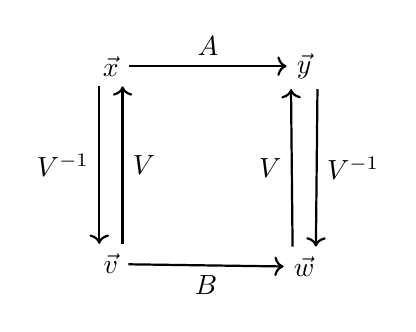
\begin{tikzpicture}[node distance = 2cm, thick]%
        \node (1) {$\vec{x}$};
        \node (2) [right=of 1] {$\vec{y}$};
        \node (3) [below=of 2] {$\vec{w}$};
        \node (4) [below=of 1] {$\vec{v}$};
        \draw[->] (1) -- node [midway,above] {$A$} (2);
        \draw[->] (1.240) -- node [midway,left]{$V^{-1}$} (4.120);
        \draw[->] (4.60) -- node [midway,right]{$V$} (1.300);
        \draw[->] (2.300) -- node [midway,right]{$V^{-1}$} (3.60);
        \draw[->] (3.120) -- node [midway,left]{$V$} (2.240);
        \draw[->] (4) -- node [midway,below] {$B$} (3);
      \end{tikzpicture}%
    \end{figure}
  }
  % % Part(c) solution
  % \sol{
  %   Start by writing $\vec{x_1}$ in terms of $\vec{z_1}$:
  %   $$ \vec{x_1} = V \vec{z_1} $$
  %   Then, apply the transformation $A$ to $\vec{x_1}$, substituting $V \vec{z_1}$ for $\vec{x_1}$:
  %   $$ \vec{x_2} = A V \vec{x_1} $$
  %   Finally, left-multiply both sides by $V^{-1}$ to change $\vec{x_2}$ to the eigenbasis:
  %   $$ \vec{z_2} = V^{-1} \vec{x_2} = V^{-1} A V \vec{z_1} $$

  %   $$A' = V^{-1} A V =
  %   \begin{bmatrix}
  %     1 & 1 \\
  %     -2 & 1
  %   \end{bmatrix}^{-1}
  %   \begin{bmatrix}
  %     3 & -1 \\
  %     -2 & 4
  %   \end{bmatrix}
  %   \begin{bmatrix}
  %     1 & 1 \\
  %     -2 & 1
  %   \end{bmatrix}
  %   $$

  %   $A'$ represents the transformation $A$ in the eigenbasis of $A$, so we know that $A'$ is the diagonal matrix:
  %   $$ A' =
  %   \begin{bmatrix}
  %     \lambda_1 & 0 \\
  %     0 & \lambda_2
  %   \end{bmatrix} =
  %   \begin{bmatrix}
  %     5 & 0 \\
  %     0 & 2
  %   \end{bmatrix} $$

  %   In general, suppose we have a linear transformation $T$ represented by a $n \times n$ matrix that transforms $\vec{u} \in \R^{n}$ to $\vec{v} \in \R^{n}$:
  %   \[
  %     \vec{v} = T\vec{u}
  %   .\]
  %   Suppose we have a basis vectors $\vec{a_1}, \cdots, \vec{a_n} \in \R^{n}$, and the vectors $\vec{u}, \vec{v}$ above are represented in this basis:
  %   \[
  %     \begin{aligned}
  %       \vec{u_a} &= u_{a_1}\vec{a_1} + \cdots + u_{a_n}\vec{a_n} \\
  %       \vec{v_a} &= v_{a_1}\vec{a_1} + \cdots + v_{a_n}\vec{a_n}.
  %     \end{aligned}
  %   \]
  %   Thus we have
  %   \[
  %     \begin{aligned}
  %       T\vec{u}          &= \vec{v} \\
  %       TA\vec{u_a}       &= A\vec{v_a} \\
  %       A^{-1}TA\vec{u_a} &= \vec{v_a}.
  %     \end{aligned}
  %   \]
  %   By pattern matching, we see that if we set $T_a = A^{-1}TA$, we get the relationship $T_a\vec{u_a} = \vec{v_a}$ in the new basis.
  %   The correspondences stated above are all represented in the following diagram:
  %   % \begin{figure}[H]
  %   %   \centering
  %   %   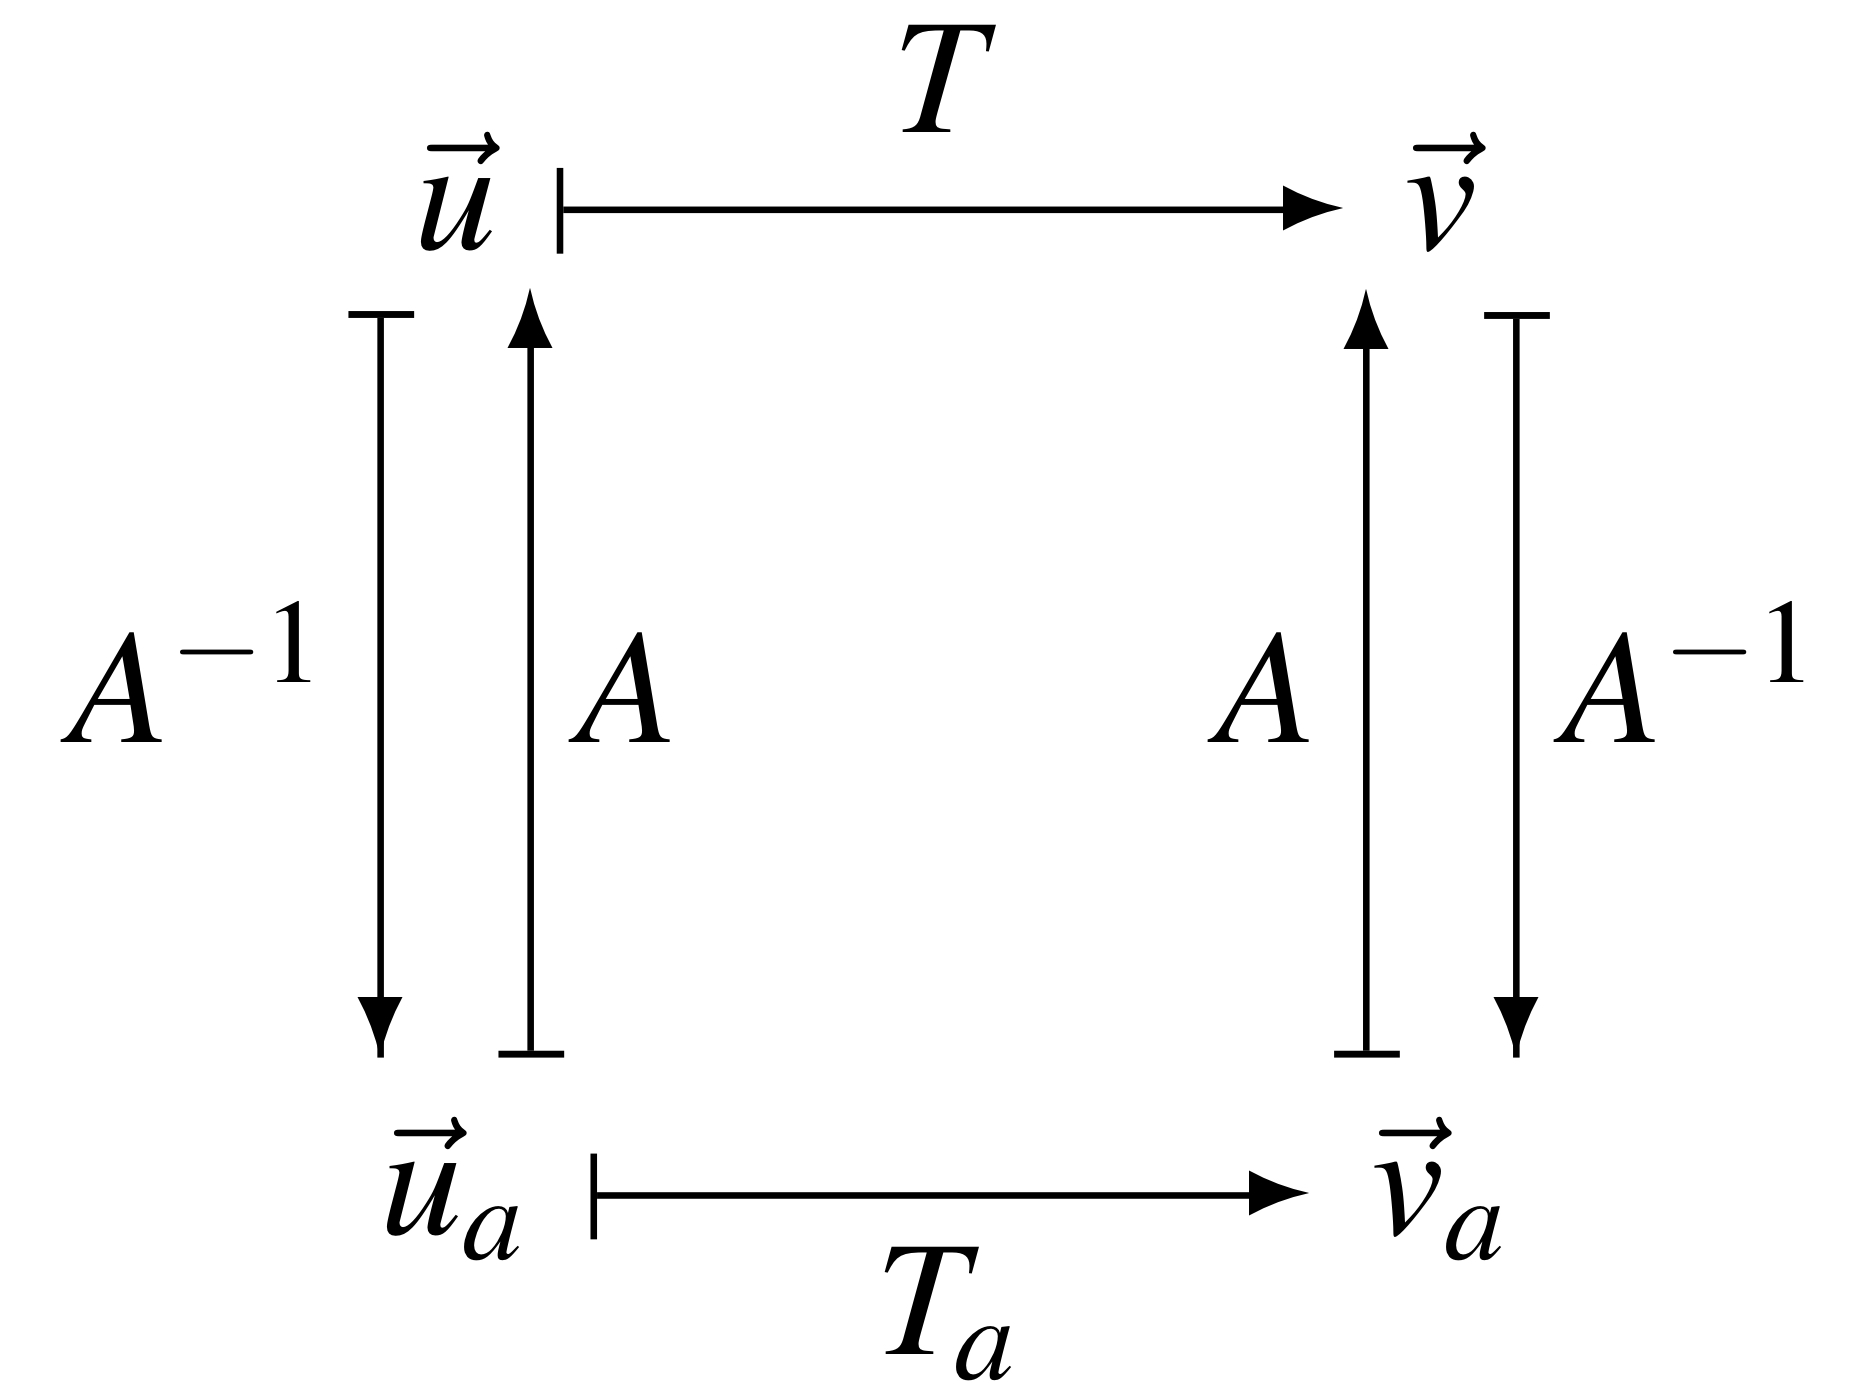
\includegraphics[scale=0.1]{\bank/statespace/figures/change_of_basis.jpg}
  %   % \end{figure}
\end{enumerate}

\newpage
% Author: Yannan Tuo, Varsha Ramakrishnan, Taejin Hwang
% Email: ytuo@berkeley.edu, vio@berkeley.edu, taejin@berkeley.edu
% Edited Lydia Lee, Spring 2019
% lydia.lee@berkeley.edu
% Edited: Justin Yu, Spring 2020
% justinvyu@berkeley.edu

\qns{Eigendecomposition and Change of Basis}

\meta{
  Please do a mini-lecture on change of basis similar to the opening paragraph of the change of coordinates question before doing this one.It is crucial that students understand change of basis, and how to convert from different bases first, before trying to understand eigendecomposition. It is up to you whether you want to mention the fact that all diagonalizable linear operators have a diagonal matrix representation given the correct choice of basis.
}

\textbf{Diagonal matrices}, matrices where all entries outside of the diagonal are zero, are often desirable since they are easy to analyze.
Determining properties such as rank and invertibility, are much simpler on a diagonal matrix as opposed to other non-diagonal matrices.
The process of \textbf{changing to a basis} in which the linear operator has a diagonal matrix representation is called \textbf{eigendecomposition} or \textbf{diagonalization.} You can think of eigendecomposition as a change of basis to one entirely made up of eigenvectors.

So what is a \textbf{change of basis}? Consider an arbitrary vector in $\mathbb{R}^2$: $\vec{x} = [ x_1 \text{ } x_2 ]^T$.
When we write a vector in this form, we are representing it as a linear combination of the \textit{standard basis} vectors for $\mathbb{R}^2$: $\vec{x} = x_1 \begin{bsmallmatrix} 1 \\ 0 \end{bsmallmatrix} + x_2 \begin{bsmallmatrix} 0 \\ 1 \end{bsmallmatrix}$. Naturally, $x_1$ and $x_2$ are the \textit{coordinates} of $\vec{x}$ in the standard basis (as you would refer to them if you graphed $\vec{x}$ on a Cartesian plane).

Now what if we wanted to represent that same vector in a different basis?
For example, say you wanted to represent the same vector $\vec{x}$ using the set of basis vectors $\vec{v_1}$ and $\vec{v_2}$.
This means that we need to find scalars $\alpha_1$ and $\alpha_2$ such that $\vec{x}$ can be written as a linear combination of these new basis vectors: $\vec{x} = \alpha_1 \vec{v_1} + \alpha_2 \vec{v_2}$.
To do this, we can just setup and solve a system of linear equations of the form:
$$\begin{bmatrix} \vec{v_1} & \vec{v_2} \end{bmatrix} \begin{bmatrix} \alpha_1 \\ \alpha_2 \end{bmatrix} = \begin{bmatrix} x_1 \\ x_2 \end{bmatrix}$$

In this problem, we'll investigate changing to and from the \textbf{eigenbasis} for the following matrix:

$$A = \begin{bmatrix}
2 & 2 \\
5 & -1
\end{bmatrix}$$

\begin{enumerate}

\qitem \textbf{Find $\lambda_1, \lambda_2$, the eigenvalues of $A$, ordered from largest to smallest.}
\ws{
\vspace{200px}
}

\meta {
  These first two parts are optional if students are comfortable with the process of finding eigenvalues and eigenspaces.
  It gives some concrete values that students can try out for the rest of the problem. If your students aren't convinced
  by $A = VDV^{-1}$, have them try out the concrete example with the numbers calculated in the first two parts.
}

\sol{
  \begin{align*}
    \text{det}(A - \lambda I) &= 0 \\
    (2 - \lambda) (-1 - \lambda) - 2(5) &= 0 \\
    \lambda^2 - \lambda - 12 &= 0 \\
    \implies \lambda_1 &= 4 \\
    \lambda_2 &= -3
  \end{align*}
}

\qitem \textbf{Find the eigenvectors $\vec{v_1}, \vec{v_2}$ corresponding to the eigenvalues.}

\ws{
\vspace{200px}
}

\sol{
  % \begin{bmatrix} 1 \\ 1 \end{bmatrix} \\ \begin{bmatrix} 1 \\ -1 \end{bmatrix}
  $$\vec{v_1} = \alpha \begin{bmatrix} 1 \\ 1 \end{bmatrix}$$
  $$\vec{v_2} = \beta \begin{bmatrix} 1 \\ -5/2 \end{bmatrix}$$
}

\end{enumerate}

With the eigenvectors we just found, define $V$ to be the matrix:
$$V = \begin{bmatrix}
\vec{v_1} & \vec{v_2}
\end{bmatrix}$$

\begin{enumerate}[resume]

\qitem Let $\widetilde{\vec{x}}$ be the coordinates of $\vec{x}$ in the eigenbasis. This means that for some arbitrary vector represented in the eigenbasis $\widetilde{\vec{x}} = \begin{bmatrix} \alpha_1 \\ \alpha_2 \end{bmatrix}$, the corresponding representation in standard coordinates is a linear combination of the columns of $V$: $\vec{x} = \alpha_1 \vec{v_1} + \alpha_2 \vec{v_2}$. \textbf{What is $\widetilde{\vec{x}}$ in terms of $V$ and $\vec{x}?$}

(\textit{Hint: Write $\vec{x}$ in terms of $V$ and $\tilde{\vec{x}}$, then go from there.})

\ws{\vspace{3em}}

\meta{
  The line $\alpha_1 \vec{v_1} + \alpha_2 \vec{v_2} = V \widetilde{\vec{x}}$ is not the most intuitive.
  It may require you showing on the board, why matrix vector multiplication can be seen as a linear combination of the columns.
}

\sol{
  $\vec{x} = \alpha_1 \vec{v_1} + \alpha_2 \vec{v_2} = V \widetilde{\vec{x}}.$ So it follows that $\widetilde{\vec{x}} = V^{-1} \vec{x}.$
}

\qitem It is often helpful to visualize the change of basis in a state diagram, where \textit{each arrow represents left-multiplying the variable it's coming out of by the corresponding matrix.} \textbf{Fill in the missing matrix operations in the state diagram based on your answer from the previous part.}

\ws {
  \begin{figure}[H]
    \centering
    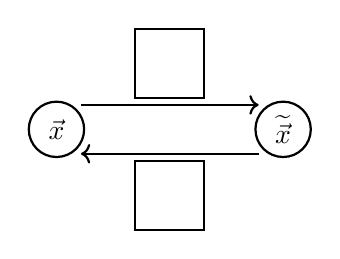
\begin{tikzpicture}[node distance = 2cm, thick,every node/.style={inner sep=0.25em,outer sep=0.25em}]%
      \node (1) [circle,draw,minimum size=2em] {$\vec{x}$};
      \node (2) [circle,draw,right=of 1,minimum size=2em] {$\widetilde{\vec{x}}$};
      \draw[->] (1.45) -- node [rectangle,draw,midway,above,minimum size=2.5em] {} (2.135);
      \draw[->] (2.225) -- node [rectangle,draw,midway,below,minimum size=2.5em] {} (1.315);
    \end{tikzpicture}%
  \end{figure}
}

\meta {
  Not everyone finds this diagram the most intuitive, but it definitely helps a large percentage of students. Stress to students that it's always better to understand the intuitive meaning behind change of basis than to remember any particular change of basis formula. This intuitive meaning is bridging between coordinate systems, which can be visualized with this diagram.
}

\sol {
  \begin{figure}[H]
  \centering
  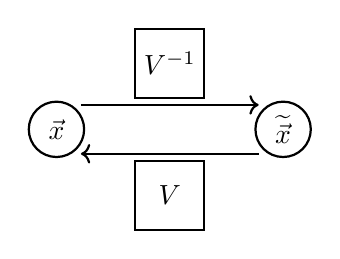
\begin{tikzpicture}[node distance = 2cm, thick,every node/.style={inner sep=0.25em,outer sep=0.25em}]%
    \node (1) [circle,draw,minimum size=2em] {$\vec{x}$};
    \node (2) [circle,draw,right=of 1,minimum size=2em] {$\widetilde{\vec{x}}$};
    \draw[->] (1.45) -- node [rectangle,draw,midway,above,minimum size=2.5em] {$V^{-1}$} (2.135);
    \draw[->] (2.225) -- node [rectangle,draw,midway,below,minimum size=2.5em] {$V$} (1.315);
  \end{tikzpicture}%
  \end{figure}
}


\qitem Now that we are able to switch back and forth between the coordinate systems, let's see how the linear transformation brought by $A$ can be viewed as a diagonal scaling transformation in the eigenbasis coordinate system.% Might be a bit confusing.

Let $\vec{y} = A \vec{x}$, and $\vec{x} = \alpha_1 \vec{v_1} + \alpha_2 \vec{v_2}$, using the same matrix $A$ and eigenvectors $\vec{v_1}, \vec{v_2}$ from before. Let $\widetilde{\vec{x}}$, $\widetilde{\vec{y}}$ be the coordinates of $\vec{x}$, $\vec{y}$ in the eigenbasis. \textbf{Find $\widetilde{\vec{x}}$ and $\widetilde{\vec{y}}$ in terms of $\alpha_1, \alpha_2, \lambda_1, \lambda_2$. What can we say about the relationship between $\widetilde{\vec{x}}$ and $\widetilde{\vec{y}}$?} % Might be confusing as to what the problem is asking compared to the next part.

(\textit{Hint}: Your answers shouldn't be in terms of the original $\vec{x}$ or $\vec{y}$.
 Use what you know about the coordinates of a vector in a certain basis; there is no need to invert any matrices or do any major computation.)

\ws {
  \vspace{200px}
}

\meta {
  Students may try to use what they found in the previous parts to multiply the vectors by $V^{-1}$. While this is technically right, make sure they understand what exactly
  that transformation is doing and why they don't need to do any matrix computation to find the coordinates of $\vec{y}$ in the eigenbasis.
}

\sol {
  $$\widetilde{\vec{x}} = \begin{bmatrix} \alpha_1 \\ \alpha_2 \end{bmatrix}$$

  \begin{align*}
    \vec{y} &= A \vec{x} \\
    &= A(\alpha_1 \vec{v_1} + \alpha_2 \vec{v_2}) \\
    &= \alpha_1 A \vec{v_1} + \alpha_2 A \vec{v_2} \\
    &= \alpha_1 \lambda_1 \vec{v_1} + \alpha_2 \lambda_2 \vec{v_2} \\
    \implies \widetilde{\vec{y}} &= \begin{bmatrix} \alpha_1 \lambda_1 \\ \alpha_2 \lambda_2 \end{bmatrix}
  \end{align*}

  This means that the matrix $D$ relating the two coordinates in the eigenbasis must be a diagonal scaling transformation, with the eigenvalues as the amount each dimension is scaled by.
}

\qitem \textbf{Find the matrix $D$ satisfying $\widetilde{\vec{y}} = D \widetilde{\vec{x}}$ in terms of $V$ and $A$.}

(\textit{Hint}: Start by writing $\vec{x}, \vec{y}$ in terms of $\widetilde{\vec{x}}$ and $\widetilde{\vec{y}}$. Refer to the state diagram from before.)

\ws{\vspace{240px}}

\meta {
  If students are comfortable with matrices representing linear transformations, you can explain this eigendecomposition as translating a linear transformation to and from the eigenbasis. For the diagonalization $A = VDV^{-1}$, left-multiplying an arbitrary vector $\vec{x}$ is equivalent to the following:

  \begin{align*}
    A \vec{x} &= VDV^{-1} \vec{x} \\
    &= VD \widetilde{\vec{x}} \\
    &= VD \begin{bmatrix} \alpha_1 \\ \alpha_2 \end{bmatrix} \\
    &= V \begin{bmatrix} \alpha_1 \lambda_1 \\ \alpha_2 \lambda_2 \end{bmatrix} \\
    &= V \widetilde{\vec{y}} \\
    &= \vec{y}
  \end{align*}
}

\sol {
  \begin{align*}
    \vec{y} &= A \vec{x} \\
    V \widetilde{\vec{y}} &= A V \widetilde{\vec{x}} \\
    \widetilde{\vec{y}} &= V^{-1} A V \widetilde{\vec{x}} \\
    \implies D &= V^{-1} A V
  \end{align*}
}

\qitem Finally, let's visualize this linear transformation $A$ from the perspective of two different coordinate systems in the state diagram below. \textbf{Fill in the missing matrix operations in the state diagram. How can you show and explain the diagonalization $A = VDV^{-1}$ (using the state diagram) and the change of basis perspective?}

\ws {
  \begin{figure}[H]
    \centering
    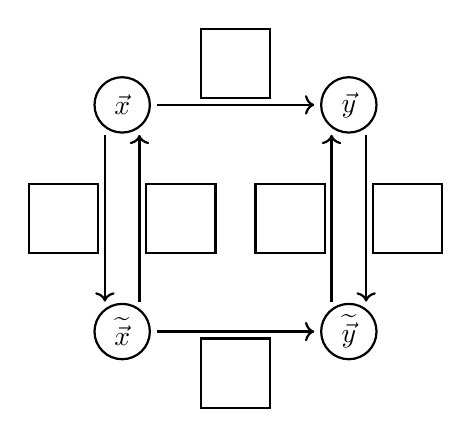
\begin{tikzpicture}[node distance = 2cm, thick, every node/.style={inner sep=0.25em,outer sep=0.25em}]%
      \node (1) [circle,draw,minimum size=2em] {$\vec{x}$};
      \node (2) [circle,draw,right=of 1,minimum size=2em] {$\vec{y}$};
      \node (3) [circle,draw,below=of 2,minimum size=2em] {$\widetilde{\vec{y}}$};
      \node (4) [circle,draw,below=of 1,minimum size=2em] {$\widetilde{\vec{x}}$};
      \draw[->] (1) -- node [rectangle,draw,midway,above,minimum size=2.5em] {} (2);
      \draw[->] (1.240) -- node [rectangle,draw,midway,left,minimum size=2.5em]{} (4.120);
      \draw[->] (4.60) -- node [rectangle,draw,midway,right,minimum size=2.5em]{} (1.300);
      \draw[->] (2.300) -- node [rectangle,draw,midway,right,minimum size=2.5em]{} (3.60);
      \draw[->] (3.120) -- node [rectangle,draw,midway,left,minimum size=2.5em]{} (2.240);
      \draw[->] (4) -- node [rectangle,draw,midway,below,minimum size=2.5em] {} (3);
    \end{tikzpicture}%
  \end{figure}
}

\sol {
  \begin{figure}[H]
    \centering
    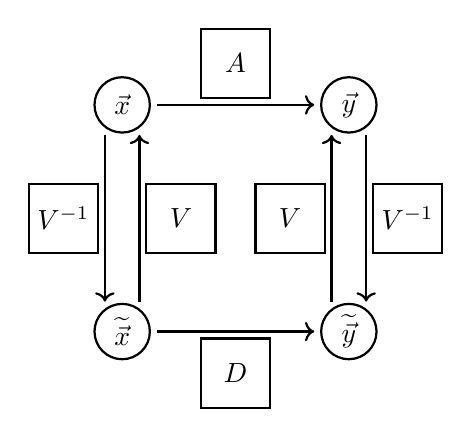
\begin{tikzpicture}[node distance = 2cm, thick, every node/.style={inner sep=0.25em,outer sep=0.25em}]%
      \node (1) [circle,draw,minimum size=2em] {$\vec{x}$};
      \node (2) [circle,draw,right=of 1,minimum size=2em] {$\vec{y}$};
      \node (3) [circle,draw,below=of 2,minimum size=2em] {$\widetilde{\vec{y}}$};
      \node (4) [circle,draw,below=of 1,minimum size=2em] {$\widetilde{\vec{x}}$};
      \draw[->] (1) -- node [rectangle,draw,midway,above,minimum size=2.5em] {$A$} (2);
      \draw[->] (1.240) -- node [rectangle,draw,midway,left,minimum size=2.5em]{$V^{-1}$} (4.120);
      \draw[->] (4.60) -- node [rectangle,draw,midway,right,minimum size=2.5em]{$V$} (1.300);
      \draw[->] (2.300) -- node [rectangle,draw,midway,right,minimum size=2.5em]{$V^{-1}$} (3.60);
      \draw[->] (3.120) -- node [rectangle,draw,midway,left,minimum size=2.5em]{$V$} (2.240);
      \draw[->] (4) -- node [rectangle,draw,midway,below,minimum size=2.5em] {$D$} (3);
    \end{tikzpicture}%
  \end{figure}

  You can explain $A = VDV^{-1}$ by just left-multiplying in the order of the arrows from $\vec{x}$ to $\vec{y}$. Again, in the change of basis perspective, $V^{-1}$ first pulls the vector $\vec{x}$ into the eigenbasis. $D$ performs the equivalent linear transformation of $A$ but in the eigen-coordinate system. Finally, $V$ brings the transformed vector back into standard coordinates.
}

% \qitem In the standard basis, we currently have the input output relation: $\vec{y} = D \vec{x}.$
% Using a change of coordinates, how can we represent our original diagonal matrix as an input-output relationship in the basis S?
% That is, if $[\vec{y}]_S = A [\vec{x}]_S,$ how would you represent $A?$

% \sol {
%   We start with the current conversion between standard and S-coordinates.
%   \begin{gather*}
%     \vec{x} = V [\vec{x}]_S, \vec{y} = V [\vec{y}]_S
%   \end{gather*}

%   Then substituting in for the original relation $\vec{y} = D \vec{x},$ we get:
%   $$V[\vec{y}]_S = D V[\vec{x}]_S$$

%   Left multiplying by $V^{-1}$ we see that:
%   $$[\vec{y}]_S = V^{-1} D V[\vec{x}]_S$$

%   So it follows that $A = V^{-1} D V$
% }

% \qitem Now we will look at the case in which we start with the matrix
% $$ A = \begin{bmatrix}
%         1 & 4 \\
%         2 & 3
%   \end{bmatrix} $$
% represented in the standard basis. What are the eigenvalues of $A?$ Order from largest to smallest.

% \sol {
%   In order to find the eigenvalues of $A,$ we look at the determinant of $A - \lambda I.$
%   $$det\mathbf{\begin{bmatrix}
%   1-\lambda & 4 \\
%   2 & 3-\lambda
%  \end{bmatrix}}  =  (1 - \lambda)(3 - \lambda) - 8 =  \lambda^2 - 4 \lambda - 5 = 0$$
%  $$ \lambda_1 = 5, \lambda_2 = -1$$
% }

% \qitem What is a basis for the eigenspace for $\lambda_1$ and $\lambda_2?$

% \sol {
%   To find the eigenspaces for $\lambda$ we compute the null-spaces of $A - \lambda I.$
%   $$A - 5I = \begin{bmatrix}
%   -4 & 4 \\
%   2 & -2
%  \end{bmatrix}$$
%  We can see that $\begin{bmatrix} 1 \\ 1 \end{bmatrix}$ is a basis for the null-space of $A - 5I.$

%  $$A + I = \begin{bmatrix}
%   2 & 4 \\
%   2 & 4
%  \end{bmatrix}$$
%  We can see that $\begin{bmatrix} -2 \\ 1 \end{bmatrix}$ is a basis for the null-space of $A + I.$
% }

% \qitem What do you notice about the eigenvalues and eigenvectors of $A?$

% \sol {
%   The eigenvectors of $A$ are the same vectors as the vectors in the basis $S.$ \\
%   The eigenvalues of $A$ have the same values as the diagonal entries of the matrix $D.$ \\
%   This should not be a coincidence. This is because $A$ is in fact a linear operator with a diagonal matrix representation "hidden" under the eigenbasis.
% }

% \qitem In the standard basis, we currently have the input output relation: $\vec{y} = A \vec{x}.$
% Using a change of coordinates, how can we represent our original diagonal matrix as an input-output relationship in the basis S?
% That is, if $[\vec{y}]_S = B [\vec{x}]_S,$ how would you represent $B?$ Try to do the calculation as well.

% \meta{
%   If you don't do end up doing the calculation, at least write out the matrices A and V as you're doing this, and state that $B = D$ at the end.
% }

% \sol {
%   We start with the current conversion between standard and S-coordinates.
%   \begin{gather*}
%     \vec{x} = V [\vec{x}]_S, \vec{y} = V [\vec{y}]_S
%   \end{gather*}

%   Then substituting in for the original relation $\vec{y} = A \vec{x},$ we get:
%   $$V[\vec{y}]_S = A V[\vec{x}]_S$$

%   Left multiplying by $V{-1}$ we see that:
%   $$[\vec{y}]_S = V^{-1} A V[\vec{x}]_S$$

%   So it follows that $B = V^{-1} A V.$ \vskip 1pt
%   However after doing the calculation, we see that $B = D!$
% }

% \qitem What is the relationship between $A, D$ and $V?$ In other words, how can you express $A$ using $D$ and $V?$

% \sol {
%   We saw from the previous part that $D = V^{-1} A V.$
%   Therefore, $A = V D V^{-1}.$
% }

% \qitem When can a matrix not be diagonalized?
% In other words, when does a linear operator not have a diagonal matrix representation?

% \sol {
%   A linear operator cannot have a diagonal matrix representation if it isn't possible to change to a basis made up of eigenvectors.
%   Remember that a change of coordinates matrix must be invertible.
%   However, if a matrix does not have $n$ linearly independent eigenvectors, then it cannot have a change of basis matrix.
% }

\end{enumerate}

\newpage
\input{\bank/vector-diff-eq/vector_diff_eq}
\newpage
\pgfplotsset{width=7cm,compat=1.16}
\usepgfplotslibrary{polar}

\qns{Complex Numbers (Optional)}

\meta{Tell students that it's not necessary to simplify some of the values as they can be quite complicated and unwieldy. For z = a + bj, you can tell students that b is scaling j, so j acts as a unit vector for the imaginary axis. Likewise, a is multiplying an implicit "1", so it is an "invisible" unit vector for the real axis}

A complex number, $z$, is composed of a real part and imaginary part.
If $z = a + bj$, then $\mathfrak{Re}(z) = a$ (the real portion equals a), and $\mathfrak{Im}(z) = b$ (the imaginary portion equals b).
Complex numbers can be expressed in two ways:

\hspace{2 em} Rectangular Form: $z = a + bj$ \hspace{14em} Polar Form: $z = re^{j\theta}$

\begin{figure}[h]
\centering
    \begin{tikzpicture}[scale=0.8, transform shape]
    \draw (0,-4)--(0,4) node[above] {$Im$} (-4,0)--(4,0) node[right] {$Re$};
    \draw[dashed] (0,0) circle (3) circle (2) circle (1);
    \draw (-1.15,0.93)--(-1.15,1.045) node[near start, fill=white] {$r = 1$};
    \draw (-1.85,1.65)--(-1.78,1.78) node[near start=3pt, fill=white] {$r = 2$};
    \draw (-2.45,2.45)--(-2.55,2.55) node[near start=3pt, fill=white] {$r = 3$};
    \draw [line width=0.25mm, blue, ->] (0,0) -- (2.4,1.3) node [below right] {};
    \draw [dotted, line width=0.25mm, blue, ->] (0,0) -- (2.4,0) node [below right]{};
    \draw [dotted, line width=0.25mm, blue, ->] (2.4,0) -- (2.4,1.3) node [below right]{};
    \draw (1.5,-0.3)--(1.6,-0.3) node[near start=3pt, fill=white] {\color{blue}$a$};
    \draw (2.7,0.6)--(2.7,0.6) node[near start=3pt, fill=white] {\color{blue}$b$};
    \draw (3.5,1.4)--(3.5,1.4) node[near start=3pt, fill=white] {\color{blue}$z = a + bj$};
    \end{tikzpicture}
\hfill
    \begin{tikzpicture}[scale=0.8, transform shape]
    \draw (0,-4)--(0,4) node[above] {$Im$} (-4,0)--(4,0) node[right] {$Re$};
    \draw[dashed] (0,0) circle (3) circle (2) circle (1);
    \draw (-1.15,0.93)--(-1.15,1.045) node[near start, fill=white] {$r = 1$};
    \draw (-1.85,1.65)--(-1.78,1.78) node[near start=3pt, fill=white] {$r = 2$};
    \draw (-2.45,2.45)--(-2.55,2.55) node[near start=3pt, fill=white] {$r = 3$};
    \draw [line width=0.25mm, blue, ->] (0,0) -- (2.4,1.3) node [below right] {};
    \draw (3.2,1.55)--(3.2,1.55) node[near start=3pt, fill=white] {\color{blue}$z = r e^{j \theta}$};
    \draw (1.2,1.0)--(1.2,1.0) node[near start=3pt, fill=white] {\color{blue}$r$};
    \draw (0.6,0.15)--(0.6,0.15) node[scale=0.9,text opacity=1, opacity=0,near start=3pt, fill=white] {\color{blue}\small$\theta$};
    \end{tikzpicture}
\end{figure}

In polar form, $r$ represents the magnitude and $\theta$ represents the angle of the complex number with respect to the origin of the complex plane.
Rectangular form makes adding and subtracting complex numbers easier; whereas, polar form makes multiplying and dividing numbers easier.
Some handy equations to switch between forms include:

\begin{center}

\begin{tabular}{ c c c }
 $\tan(\theta) = \frac{b}{a}$ & $r = |z| = \sqrt{a^2 + b^2}$ \\ \\
 $\sin(\theta) = \frac{b}{|z|}$ & $\cos(\theta) = \frac{a}{|z|}$ \\  \\
\end{tabular}

\end{center}

\vspace{-15px}

\begin{enumerate}
\qitem \textbf{Use the formulas given above to convert between polar and rectangular form.}

\begin{enumerate}
\qitem Convert $10 + 12j$ to polar form.

\ws {
    \vspace{75px}
}

\sol{
$z = a + bj$. We can go from rectangular form to polar form by using the equation $z = |z|e^{j\theta}$, where $|z| = \sqrt{a^2 + b^2}$ and $\theta = \angle z = \atan2(b, a)$.
$$ z = 10 + 12j $$
$$ |z| = \sqrt{10^2 + 12^2} = \sqrt{244}$$
%$$ \angle z = \tan^{-1}(\frac{12}{10})$$
$$ \angle z = \atan2(12, 10)$$
$$ z = \sqrt{244}e^{j \, {\atan2(12/10)}} \approx 15.620e^{0.876j}$$
}

\qitem Convert $22e^{23j}$ to rectangular form.

\ws {
    \vspace{75px}
}

\sol{
Conversely, for $z = |z|e^{j\theta}$, we can go from polar form to rectangular form by using the equation $z = a + bj$, where $a = |z|\cos(\theta)$ and $b = |z|\sin(\theta)$. So, \\
$$ a = 22\cos(23) $$
$$ b = 22\sin(23) $$
$$ z = 22\cos(23) + 22j \sin(23) \approx -11.722 + -18.617j$$
}
\end{enumerate}


\qitem \textbf{Plot the following on a polar grid:}
\begin{enumerate}

\qitem {2}

\sol {
\newline
\begin{tikzpicture}
    \draw (0,-4)--(0,4) node[above] {$Im$} (-4,0)--(4,0) node[right] {$Re$};
    \draw[dashed] (0,0) circle (3) circle (2) circle (1);
    \draw (-1.15,0.93)--(-1.15,1.045) node[near start, fill=white] {$r = 1$};
    \draw (-1.85,1.65)--(-1.78,1.78) node[near start=3pt, fill=white] {$r = 2$};
    \draw (-2.45,2.45)--(-2.55,2.55) node[near start=3pt, fill=white] {$r = 3$};
    \draw [line width=0.25mm, blue, ->] (0,0) -- (2,0) node [below right] {2};
\end{tikzpicture}
}

\qitem {2j}

\sol {
\newline
\begin{tikzpicture}
    \draw (0,-4)--(0,4) node[above] {$Im$} (-4,0)--(4,0) node[right] {$Re$};
    \draw[dashed] (0,0) circle (3) circle (2) circle (1);
    \draw (-1.15,0.93)--(-1.15,1.045) node[near start, fill=white] {$r = 1$};
    \draw (-1.85,1.65)--(-1.78,1.78) node[near start=3pt, fill=white] {$r = 2$};
    \draw (-2.45,2.45)--(-2.55,2.55) node[near start=3pt, fill=white] {$r = 3$};
    \draw [line width=0.25mm, blue, ->] (0,0) -- (0,2) node [below right] {2j};
\end{tikzpicture}

}

\qitem {2 + 2j}

\sol {
\newline
\begin{tikzpicture}
    \draw (0,-4)--(0,4) node[above] {$Im$} (-4,0)--(4,0) node[right] {$Re$};
    \draw[dashed] (0,0) circle (3) circle (2) circle (1);
    \draw (-1.15,0.93)--(-1.15,1.045) node[near start, fill=white] {$r = 1$};
    \draw (-1.85,1.65)--(-1.78,1.78) node[near start=3pt, fill=white] {$r = 2$};
    \draw (-2.45,2.45)--(-2.55,2.55) node[near start=3pt, fill=white] {$r = 3$};
    \draw [line width=0.25mm, blue, ->] (0,0) -- (2,2) node [below right] {2 + 2j};
    \draw [dotted, line width=0.25mm, blue, ->] (0,0) -- (2,0) node [below right] {};
    \draw [dotted, line width=0.25mm, blue, ->] (2,0) -- (2,2) node [below right] {};
\end{tikzpicture}

}

\ws{
\begin{tikzpicture}
    \draw (0,-4)--(0,4) node[above] {$Im$} (-4,0)--(4,0) node[right] {$Re$};
    \draw[dashed] (0,0) circle (3) circle (2) circle (1);
\end{tikzpicture}
}

\end{enumerate}

\qitem \textbf{Calculate the magnitude and phase of the following:}
\meta {
    Clarify to students that the magnitude of a complex number is $|a + bj| = \sqrt{a^2 + b^2}$, and the phase is $\theta = \text{atan2}(a ,b)$.
}

\begin{enumerate}

\qitem {2}

\ws{
  \vspace{75px}
}

\sol {
$$z = 2 + 0j.$$
$$|z| = \sqrt{2^2 + 0^2} = 2.$$
$$\angle z = \angle 2 = 0 \, \text{rad}. $$
}

\qitem $\frac{2}{2j}$

\ws{
  \vspace{75px}
}

\sol {
$$ z = \frac{2}{2j} = (\frac{1}{j})(\frac{j}{j}) = \frac{j}{j^2} = -j = 0 - 1j.$$
$$|z| = \sqrt{0^2 + (-1)^2} = 1.$$
$$\angle z = \angle -j = \frac{3\pi}{2} \, \text{rad}.$$
}

\qitem $\frac{3j}{5}$

\ws{
  \vspace{75px}
}

\sol {
$$z = 0 + \frac{3}{5}j.$$
$$|z| = \sqrt{0^2 + \frac{3}{5}^2} = \frac{3}{5}.$$
$$\angle z = \angle \frac{3}{5}j = \frac{\pi}{2} \, \text{rad}.$$
}

\qitem $\frac{1+2j}{9+7j}$

\ws{
  \vspace{75px}
}

\sol {
$$z = \frac{1+2j}{9+7j} = \frac{z_a}{z_b}.$$
$$|z| = \frac{|z_a|}{|z_b|} = \frac{\sqrt{1^2 + 2^2}}{\sqrt{9^2 + 7^2}} = \frac{\sqrt{5}}{\sqrt{130}}. \approx 0.196.$$
$$\angle z = \angle z_a - \angle z_b = \atan2(2, 1) - \atan2(7, 9)) = 1.107 + 0.661 \approx 1.768 \, \text{rad}.$$
}

\end{enumerate}


\qitem \textbf{Show that $\frac{1}{j} = -j$.}

\ws{
  \vspace{75px}
}

\sol{
The key is to multiply the left-hand side of the equation by $\frac{j}{j}$: \\
$$\frac{1}{j} = \frac{1 * j}{j * j} = \frac{j}{j^2}$$
$$= \frac{j}{-1} = -j$$
}

\end{enumerate}

A complex number, $z = a + bj$ has a \textbf{complex conjugate}, $\overline{z} = a - bj$. In polar coordinates, the equivalent expression is $\overline{re^{j\theta}} = re^{-j\theta}$.

Note that the sum of a complex number and its conjugate is always purely real, but the difference between a complex number and its conjugate is always purely imaginary.

\begin{enumerate}[resume]

\qitem \textbf{Prove graphically that the sum of any complex number and its conjugate is always real.} \textit{Try plotting an an arbitrary complex number and its conjugate.}

\ws{
    \vspace{140px}
}

\sol{
For complex number $z = a + bj$, its conjugate is $\bar{z} = a - bj$. If we add these two together, we get $z + \bar{z} = a + bj + a - bj = 2a + 0j$. The imaginary components cancel out exactly, so the resulting sum is always entirely real. This is illustrated by the following graph for $z = 1 + 1j$ and $\bar{z} = 1 - 1j$:

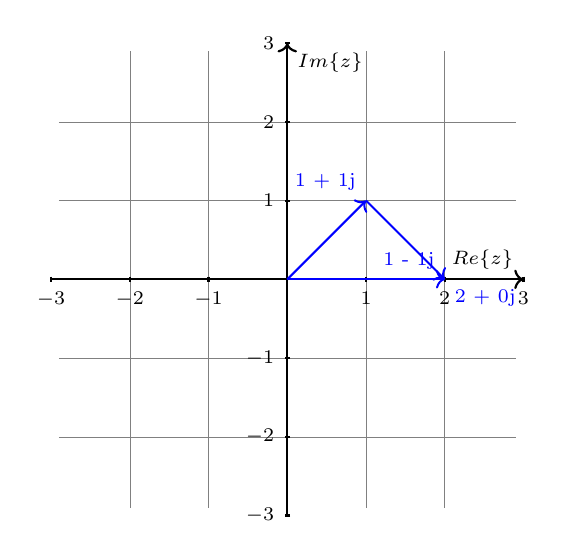
\begin{tikzpicture}
    \begin{scope}[thick,font=\scriptsize]
    \draw[step=1cm,gray,very thin] (-2.9,-2.9) grid (2.9,2.9);
    \draw [->] (-3,0) -- (3,0) node [above left]  {$Re\{z\}$};
    \draw [->] (0,-3) -- (0,3) node [below right] {$Im\{z\}$};

    \foreach \x in {-3, -2, -1, 1, 2, 3}
       \draw (\x cm,1pt) -- (\x cm,-1pt) node[anchor=north] {$\x$};
    \foreach \y in {-3, -2, -1, 1, 2, 3}
        \draw (1pt,\y cm) -- (-1pt,\y cm) node[anchor=east] {$\y$};


    \draw [line width=0.25mm, blue, ->] (0,0) -- (1,1) node [above left] {1 + 1j};
    \draw [line width=0.25mm, blue, ->] (1,1) -- (2,0) node [above left] {1 - 1j};
    \draw [line width=0.25mm, blue, ->] (0,0) -- (2,0) node [below right] {2 + 0j};
    \end{scope}
\end{tikzpicture}

}

\qitem Recall that Euler's Formula states that $e^{j\theta} = \cos(\theta) + j\sin(\theta)$.

\textbf{Using Euler's identity, show the following identities}, which show that sinusoids are sums of complex exponentials:

\begin{align*}
    \cos(\theta) = \frac{e^{j\theta} + e^{-j\theta}}{2} \\
    \sin(\theta) = \frac{e^{j\theta} - e^{-j\theta}}{2j}
\end{align*}

\sol{

  $$e^{j\theta} = \cos(\theta) + j\sin(\theta)$$

  Note that $e^{j\theta}$ has the complex conjugate $e^{-j\theta}$, which means:

  $$e^{-j\theta} = \cos(\theta) - j\sin(\theta)$$
  $$e^{j\theta} +  e^{-j\theta} = \cos(\theta) + j\sin(\theta) + \cos(\theta) - j\sin(\theta)$$
  $$e^{j\theta} +  e^{-j\theta} = 2\cos(\theta)$$
  $$cos(\theta) = \frac{1}{2}(e^{j\theta} +  e^{-j\theta})$$

  We can also notice that this is true because $cos$ is an even function and $sin$ is an odd function, which gives the properties
  $cos(-\theta) = cos(\theta)$ and $sin(-\theta) = -sin(\theta)$.

  A similar approach can be used to find $sin(\theta)$:

  \begin{align*}
    e^{j\theta} - e^{-j\theta} &= cos(\theta) + jsin(\theta) - (cos(\theta) - jsin(\theta)) \\
    &= 2jsin(\theta) \\
    \implies sin(\theta) &= \frac{e^{j\theta} - e^{-j\theta}}{2j}
  \end{align*}

}

\end{enumerate}

\newpage


\end{qunlist}

\end{document}


